\documentclass[journal,a4paper,twoside]{sty/IEEEtran}

%% Based on bare_jrnl.tex V1.3 2007/01/11 by Michael Shell (requires IEEEtran.cls version 1.7 or later) 

\usepackage[utf8]{inputenc}
\usepackage[slovene]{babel}
\usepackage{sty/EVrevija}

% *** GRAPHICS RELATED PACKAGES ***
\usepackage[pdftex]{graphicx}
\graphicspath{ {./Pictures/} }

% Include all other packages here
\usepackage{textcomp} % need for \textmu
\usepackage{setspace}
\usepackage{color}
\definecolor{light-gray}{gray}{0.95}
%\usepackage{listings} % za vključevanje kode
%\usepackage{hyperref}
%\usepackage{amsmath}
%\usepackage{amsthm}
%\usepackage{amssymb}

% correct bad hyphenation here
%\hyphenation{op-tical net-works semi-conduc-tor}

\begin{document}

% naslov prispevka, lahko uporabite en linebreak \\
\title{Analiza porazdeljenega programskega jezika Julia in primerjava z dobro znanimi alternativami}

\authors{Jan Pelicon, Blaž Rojc}
\address{Univerza v Ljubljani, Fakulteta za računalništvo in informatiko, Večna pot 113, 1000 Ljubljana, Slovenija}

\abstract{TODO}

\keywords{primerjava programskih jezikov, porazdeljeni programski jeziki, hitrost izvajanja, prijaznost do uporabnika}

%\received{19. oktober, 2010} % datum sprejema članka, lahko pustite prazno
%\review{4. februar, 2011}    % datum odobritve članka, pustite prazno

% Priimki avtorjev in kratek naslov članka za tekočo glavo
\markboth{Pelicon, Rojc}{Analiza in primerjava jezika Julia}

% make the title area
\maketitle

\IEEEpeerreviewmaketitle

% Naslov in kratek povzetek v angleščini
\english{Analisys and comparison of the Julia programming language}
{TODO}

\section{Uvod}

Porazdeljeno programiranje predstavlja težavo, s katero se večina programerjev nerada spoprijema.
V čist, striktno determinističen tok programiranja vnaša nepredvidljivost, simultane dogodke, neurejenost in kup varnostnih ter pravilnostnih lukenj.
K zahtevnosti programiranja pa pripomore tudi slaba podprtost porazdeljenega programiranja v bolj permisivnih programskih jezikih - tako Python kot
	JavaScript zahtevata daljšo poglobitev v njune sisteme, ki omogočajo distribucijo problemov po več jedrih ali procesorjih, poleg tega pa zaradi
	svojih omejitev ne morata omogočiti tako nizkonivojnega nadzora kot C.

Tu vstopi Julia, dinamičen, prevajan jezik, prvotno namenjen potrebam numerične analize in računske znanosti, a primeren za obilico problemov, kjer je
	hitrost izvajanja tako pomemben faktor kot enostavnost programiranja.\cite{julia-site}
Obljublja enostavno in učinkovito distribucijo dela, hkrati pa ohranja prijaznost do uporabnika.

\section{Jezik}

Julia predstavlja zanimivo sredino med hitrostjo C-ja in prijaznostjo do uporabnika raznih dinamičnih programskih jezikov, kot so Python, JavaSript,
	MATLAB, Lua, ...

Julia se pred izvajanjem optimizira in prevede v strojno kodo z uporabo programske opreme LLVM\footnote{http://llvm.org/}.
To omogoča učinkovito izrabo pomnilnika in procesorskega časa, posledično pa tvorbo programov, ki se v hitrosti približajo ekvivalentni implementaciji v
	jeziku C.\cite{julia-benchmarks}

Je dinamičen programski jezik v polnem pomenu besedne zveze.
Med drugim omogoča dinamično izpeljavo podatkovnih tipov, modificiranje in izvajanje kode iz besedilnih nizov,\cite{julia-metaprogramming} refleksijo, makre in večmetodnost
	funkcij.

V času pisanja tega dokumenta je jezik tudi že dosegel različico 1.0, kljub temu pa še ni popolnoma stabilen.
Kot bo opisano kasneje ostaja še velik del obljubljene funkcionalnosti neimplementirane, medtem ko ima stabilnost in hitrost obstoječe kode višjo
	prioriteto.

\section{Porazdeljeno računanje}

Julia podpira več oblik delitve dela.
Osredotočili se bomo na metode najpodobnejše tistim, ki smo jih obravnavali pri predmetu PS: eksplicitna delitev dela med procesorska jedra in pošiljanje
	dela koprocesorjem - GPE.

Julia v teoriji podpira delitev dela med procesorska jedra na več načinov, ki se večinoma delijo v dve skupini, na osnovi niti in na osnovi procesov.

Večnitenje je v Julii eksperimentalna funkcija.
Uporabnost je v času pisanja zelo omejena, na voljo sta le makra “@threads”, ki na več nitih paralelno izvede “for” zanko, in “@threadcall”, ki funkcijo v
	jeziku C pokliče v ločeni niti.\cite{julia-multithreading}
Druga možnost zahteva pisanje dela programa v različnem programskem jeziku in se ji bomo izognili.
Prva pa omogoča določeno stopnjo paralelizacije, kljub temu da morda ni tako učinkovita kot v drugih programskih jezikih.

Večprocesnost je veliko bolj fleksibilna možnost.
Procesi se v Julii lahko dodajajo poljubno med izvajanjem, komunikacija pa poteka prek klicev iz glavnega procesa v ostale.
Največja ovira tega pristopa pa je potreba po eksplicitnem podajanju podatkov med procesi, ki poleg dodane kompleksnosti prinaša še dodatno zahtevnost
	izvajanja in počasnejše računanje.

\section{Primerjava z jezikom Python}

Med dinamičnimi programskimi jeziki po popularnosti trenutno kraljuje Python.\cite{python-tiobe}\cite{python-pypl}
Je anekdotno eden najlažjih jezikov za popolne začetnike, omogoča pa tudi reševanje kompleksnejših problemov s širokim naborom javno dostopnih knjižnic -
	modulov.\cite{python-pypi}

Njegova največja hiba je relativna počasnost.
Python je interpretiran jezik, ki se najprej prevede v bitno kodo, nato pa izvaja v virtualnem stroju.
Posledično se kompleksni programi izvajajo veliko počasneje kot v C-ju.

Julia ohranja večino prednosti Pythona, predvsem dinamičnost in prijaznost do programerja, prinese pa prednost hitrega izvajanja neposredno prevedene
	kode.

Na žalost Julia ne uživa take stopnje podpore kot Python glede obstoječih knjižnic, kar pa je posledica relativne novosti jezika in pomanjkanja izkušenih,
	zavzetih programerjev.
K večji sprejetosti jezika naj bi v prihodnosti pripomogla tudi večja zanesljivost, ki naj bi prišla z uporabo jezika v večjih projektih.

\subsection{Python multiprocessing}

Za deljenje dela med jedra sta na voljo v Pythonu modula “multiprocessing”\footnote{https://docs.python.org/3.7/library/multiprocessing.html} in
	“threading”\footnote{https://docs.python.org/3.7/library/threading.html}, a na žalost se zaradi globalnega zaklepanja interpreterja
	(GIL)\cite{python-gil} v CPython implementaciji lahko izvaja naenkrat le koda ene niti v vsakem Python procesu.
Za učinkovito deljenje dela moramo torej uporabiti modul “multiprocessing”.
Ta nam omogoča zaganjanje poljubnega števila procesov in deljenje podatkov med njimi.

Tako kot v drugih programskih jezikih je tudi v Pythonu delo s procesi precej počasnejše kot z nitmi, ampak dokler je globalni zaklep prisoten, nimamo
	možnosti izbire.

\section{Primerjava z jezikom C/C++}

TODO

\subsection{pthreads}

TODO

\subsection{OpenMP}

TODO

\section{Algoritma}

Za primerjavo jezikov sva implementirala dva algoritma.

Prvi, Adaptive Quick Sort je paralelna implementacija sortirnega algoritma Quick Sort.
Zasnovan je tako, da paralelno izvede čim večji del računanja, tudi deljenje in združevanje podatkov.

Drugi simulira JPEG kompresijo.
Izvaja se na grafični kartici prek knjižnic OpenCL in CUDAnative.

\subsection{Adaptive Quick Sort}

Veliko vzporednih implementacij algoritma Quick Sort paralelizira le sortiranje, ne pa tudi deljenja in združevanja podatkov.
Adaptive Quick Sort porazdeli vse, kar omogoča hitrejše izvajanje pri zelo velikih naborih podatkov.

Idejno se vsak korak algoritma izvede v 3 delih.
Naj bo “n” število podatkov v tabeli, “t” pa število niti oz. procesov, ki jih ima algoritem na voljo.
V prvem delu se tabela razdeli na t delov in določi se pivotni element:

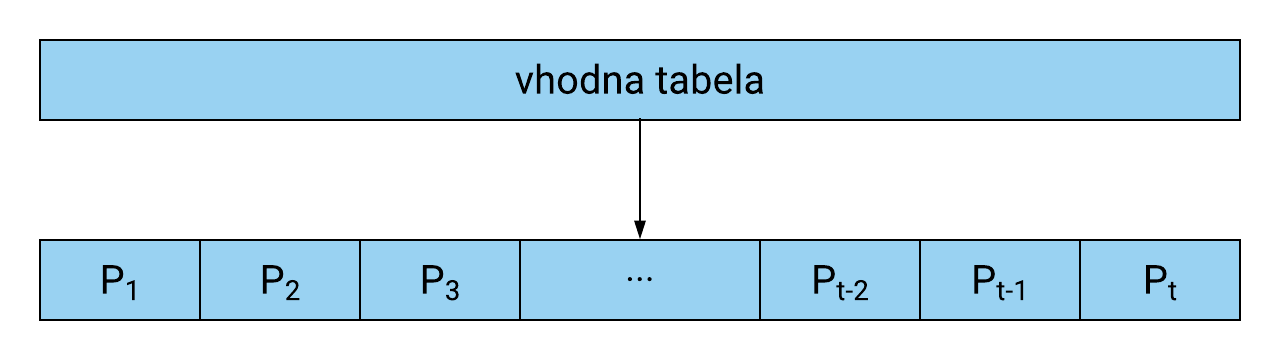
\includegraphics[width=0.45\textwidth]{aqs_diag_1}

Nato vsaka nit “in-place” razdeli svoj del na elemente manjše ali enake pivotu (L) ter elemente večje ali enake pivotu (H):

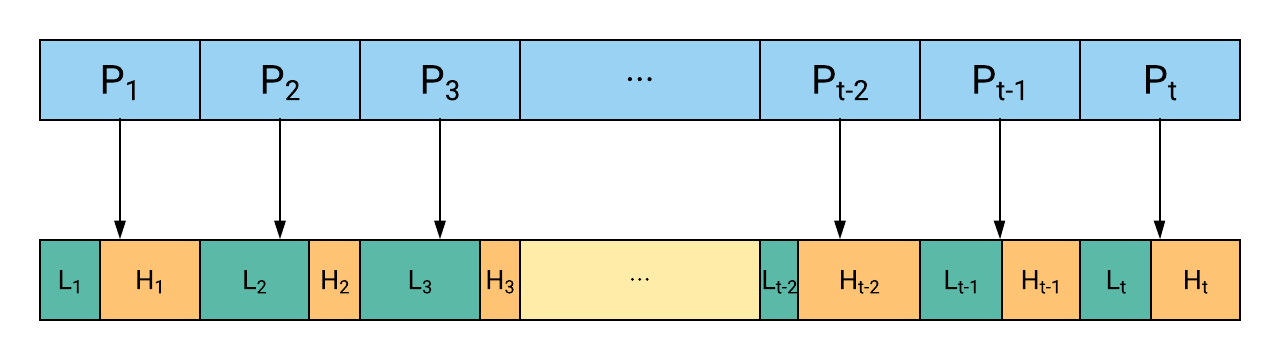
\includegraphics[width=0.45\textwidth]{aqs_diag_2}

Vse niti se nato uporabijo za premik “spodnjih” delov na začetek in “zgornjih” delov na konec tabele, vsaka nit premakne svoj kos L in kos H:

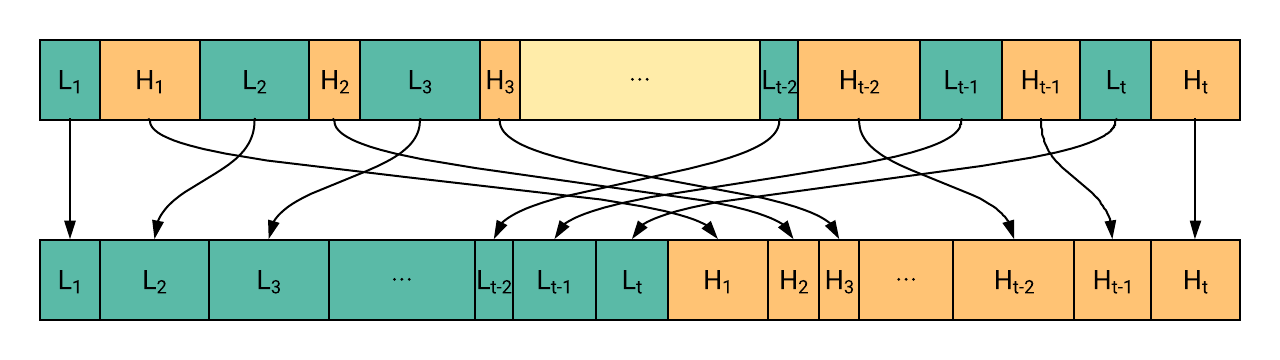
\includegraphics[width=0.45\textwidth]{aqs_diag_3}

Na koncu koraka se rekurzivno na obeh novo ustvarjenih delih tabele kliče naslednji korak v dveh ločenih nitih, vsaka dobi del nabora niti za delo:

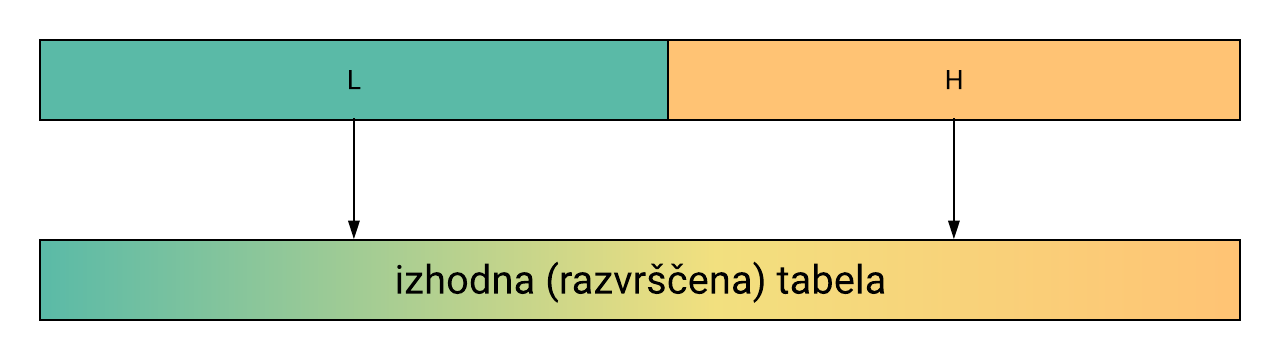
\includegraphics[width=0.45\textwidth]{aqs_diag_4}

Po koncu vseh rekurzivnih klicev je tabela sortirana.
Če je v nekem koraku na voljo le ena nit, se v tej niti izvede navaden Quick Sort.

Ta implementacija zahteva relativno veliko koordinacije med nitmi in usklajevanja velikosti delov.
Posledično zahteva več premisleka in dela kot le paralelizacija zanke.
Zaradi tega ta algoritem pokaže prednosti in slabosti jezikov ko pride do možnosti paralelizacije.

\subsection{JPEG}

Format JPEG\footnote{https://en.wikipedia.org/wiki/JPEG} za zmanjševanje količine podatkov, ki ga slike zasedajo, izrablja lastnosti človeškega vida -
	ljudje težje zaznamo spremembe pri visokofrekvenčnih komponentah slike kot pri nizkofrekvenčnih.

Kodiranje je sestavljeno iz treh glavnih delov, preslikave 8x8 kosov slike v frekvenčno domeno, kvantizacije in končnega stiskanja.

Preslikava je navadno diskretna kosinusna transformacija.[x]
Ta je implementirana kot množenje matrike vhodnih podatkov z matriko realnih koeficientov.

Kvantizacija poteka v treh korakih.
Najprej se podatki pomnožijo s kvantizacijsko matriko.
Ta določa, katere frekvence naj se bolje ohranijo.
Nato se elementi matrike zaokrožijo na cela števila med -128 in 127.
Nazadnje pa se še matrika pretvori v vektor dolžine 64 prek poševnega cik-cak vzorca:

\begin{figure}[h]
\centering
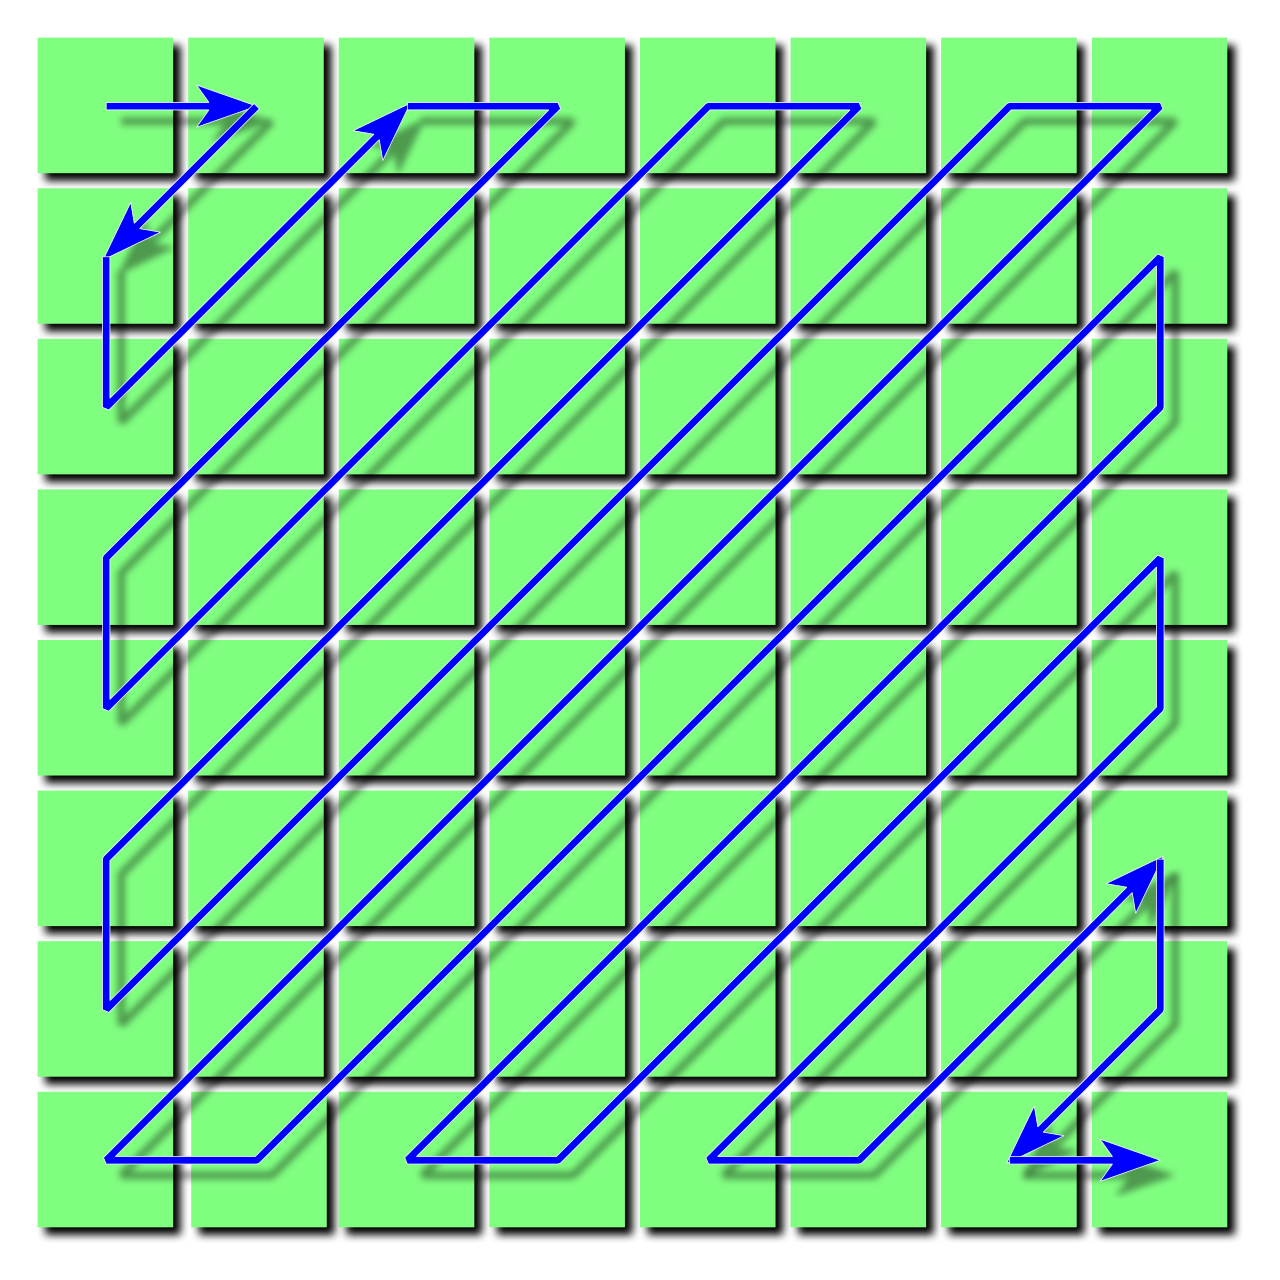
\includegraphics[width=0.35\textwidth]{jpeg_zigzag}
\caption{vir: Wikipedia}
\end{figure}

Končno stiskanje je brez izgub.
Navadno se uporablja Huffmanovo kodiranje.\footnote{https://en.wikipedia.org/wiki/Huffman\_coding}
Pri dobro izbrani kvantizacijski matriki se večina ničelnih elementov nahaja na koncu vektorja, kar lahko uporabimo, da podatke še bolj stisnemo.

Preslikava in prva dva koraka kvantizacije sta zelo primerna za izvajanje na GPE.
Algoritem simulira popačenje, ki se pojavi pri stiskanju, tako, da izvede DCT, množenje s kvantizacijsko matriko in zaokroževanje, nato pa izvede obraten
	postopek, podatke množi z inverzom kvantizacijske matrike in izvede inverzen DCT.

Ta algoritem je relativno enostaven pri implementaciji, je pa dovolj zahteven, da prikaže razlike med hitrostmi prevajanja in izvajanja programov na GPE
	med različnimi jeziki.

\section{Okolje}

Testiranje se je izvajalo na namiznem računalniku s procesorjem AMD Ryzen Threadripper 1920X na tovarniško nastavljeni hitrosti, 32 GB pomnilnika s hitrostjo
	3000 MHz in grafično kartico Nvidia GeForce GTX 1080 Ti.
Nameščen je bil operacijski sistem Windows 10 - 64 bit, različica 1809.

Programi v jeziku C/C++ so se prevajali in zaganjali v programskem okolju Microsoft Visual Studio 2017 z nastavitvami za “pthreads”, “OpenMP” in “OpenCL”
	kot je zapisano v navodilih za vaje pri predmetu Porazdeljeni sistemi.

Program v jeziku Python se je zaganjal v ukaznem pozivu Powershell, Python verzija 3.7.1 64 bit, numpy verzija 1.15.4.

Programi v jeziku Julia so se zaganjali v ukaznem pozivu Powershell, Julia verzija 1.0.3 64 bit, CUDAnative verzija 0.9.1.

\section{Analiza hitrosti}

\subsection{Adaptive Quick Sort}

Algoritem očitno izpostavi obseg razlik hitrosti posameznih jezikov in kako velikost podatkov vpliva nanje.
Programi so bili testirani na eksponento povečujoči tabeli naključno generiranih predznačenih 64-bitnih števil.
Za vsako velikost se je vsak program izvedel petkrat, vsakokrat z na novo generiranimi števili.
Največja tabela je vsebovala 200 milijonov elementov.
Končne vrednosti so povprečja petih izvajanj.

Vsak program je bil spisan na način, ki je minimiziral število nepotrebnih dostopov do pomnilnika in hkrati kar najbolje sledil prej opisanemu načrtu.
V primeru Pythona in Julie je jezik omejeval ta aspekt optimizacije, kar pa bo obravnavano kasneje.

Med pthreads in OpenMP je razlika največja pri majhnih tabelah, kjer je OpenMP veliko hitrejši.
Ta razlika se bolj ali manj izniči pri tabelah z več kot 20 milijoni elementov.

[graf primerjave pthreads, OpenMP]

Julia je le slabo magnitudo počasnejša.
Za majhne tabele je skoraj tako hitra kot pthreads.
Med 2 in 20 milijoni elementov počasi izgublja hitrost.
Pri 200 milijonih pa nastopi težava s količino pomnilnika, zato se izvajanje še dodatno upočasni.

[graf primerjave C++, Julia]

Python je od vseh jezikov najpočasnejši.
Pri 100 milijonih elementov doseže razmerje časa izvajanja v Pythonu s časom izvajanja s pthreads faktor 250.
Zaradi zelo dolgega časa testiranja pri tabeli velikosti 100 milijonov - približno 1 uro in 15 minut - se za 200 milijonov elementov ni testiralo.

[graf primerjave vseh]

\subsection{JPEG}

TODO

\section{Zahtevnost in izkušnja programiranja}

Hitrost izvajanja je le ena plat zgodbe.
Vse privarčevane sekunde ne pomenijo nič, če mora programer ure in ure razhroščevati težave brez ali s slabimi sporočili napak.

\subsection{C/C++}

TODO

\subsection{Python}

TODO

\subsection{Julia}

TODO

\section{Sklep}

TODO

\begin{thebibliography}{99}

% članek na spletni strani: \bibitem{tag} Avtor. (leto). Naslov. \emph{Stran/publikacija}. [Online] Dosegljivo: url. [Dostopano \today].
% študija: \bibitem{tag} Avtor, ``Naslov''. Institucija, (št.poročila, datum).

\bibitem{julia-site} The Julia Language. [Online] Dosegljivo: \mbox{https://www.julialang.org/}. [Dostopano \today].

\bibitem{julia-benchmarks} Julia Micro-Benchmarks. [Online] Dosegljivo: \mbox{https://www.julialang.org/benchmarks/}. [Dostopano \today].

\bibitem{julia-metaprogramming} Metaprogramming. \emph{The Julia Language}. [Online] Dosegljivo:
	https://docs.julialang.org/\allowbreak en/v1/manual/\allowbreak metaprogramming/index.html. [Dostopano \today].
	
\bibitem{julia-multithreading} Multi-Threading (Experimental). \emph{The Julia Language}. [Online] Dosegljivo:
	https://docs.julialang.org/\allowbreak en/v1/\allowbreak manual/parallel-computing/\allowbreak index.html\allowbreak \#Multi-Threading-
	(Experimental). [Dostopano \today].
	
\bibitem{python-tiobe} TIOBE Index for January 2019. \emph{TIOBE Index}. [Online] Dosegljivo: https://www.tiobe.com/tiobe-index/. [Dostopano \today].

\bibitem{python-pypl} Pierre Carbonnelle (2018). PYPL PopularitY of Programming Language. [Online] Dosegljivo: http://pypl.github.io/PYPL.html.
	[Dostopano \today].

\bibitem{python-pypi} The Python Package Index. [Online] Dosegljivo: https://pypi.org/. [Dostopano \today].

\bibitem{python-gil} Global Interpreter Lock. \emph{Python Wiki}. [Online] Dosegljivo: https://wiki.python.org/moin/GlobalInterpreterLock.
	[Dostopano \today].

\end{thebibliography}

% that's all folks
\end{document}
